\documentclass[tikz, border=5pt]{standalone}
\usepackage{pgfplots}
\pgfplotsset{compat=1.18}

\begin{document}

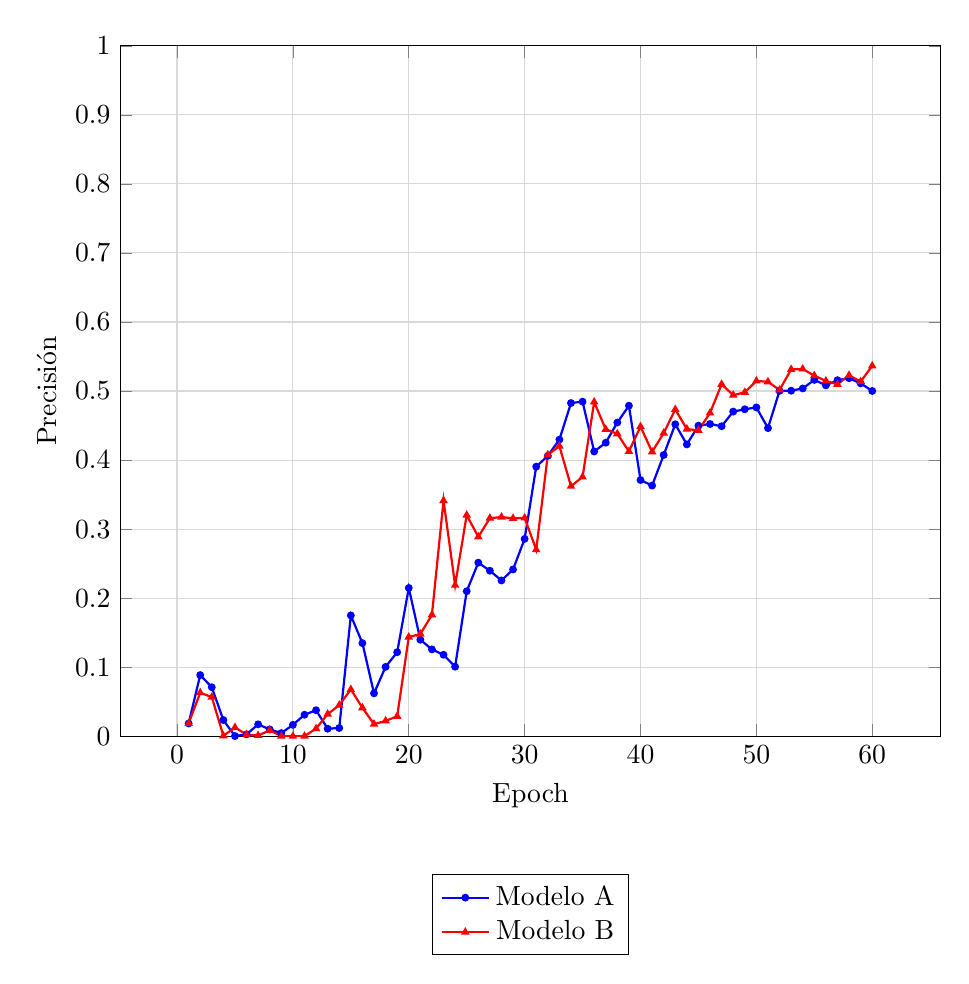
\begin{tikzpicture}
\begin{axis}[
    width=12cm,
    xlabel={Epoch},
    ylabel={Precisión},
    ymin=0, ymax=1,
    grid=both,
    grid style={gray!30},
    legend style={at={(0.5,-0.2)}, anchor=north, legend columns=1},
]

% yolo11l_e60_b16_s42_box7.5_8fb4a

\addplot[
    thick,
    mark=*,
	mark size = 1pt,
    color=blue,
]
coordinates {
    (1,0.01853) (2,0.08859) (3,0.07101) (4,0.0234) (5,0.00032)
    (6,0.00273) (7,0.01728) (8,0.00988) (9,0.00457) (10,0.01654)
    (11,0.0311) (12,0.0377) (13,0.01091) (14,0.01191) (15,0.17496)
    (16,0.13483) (17,0.06218) (18,0.10049) (19,0.1217) (20,0.21482)
    (21,0.13978) (22,0.12581) (23,0.11803) (24,0.10075) (25,0.21003)
    (26,0.2514) (27,0.23975) (28,0.22564) (29,0.24158) (30,0.28589)
    (31,0.39045) (32,0.40618) (33,0.42968) (34,0.4826) (35,0.48465)
    (36,0.41242) (37,0.42516) (38,0.45438) (39,0.47876) (40,0.37111)
    (41,0.36308) (42,0.40734) (43,0.45184) (44,0.42268) (45,0.44984)
    (46,0.45224) (47,0.44904) (48,0.47023) (49,0.47357) (50,0.47625)
    (51,0.44628) (52,0.50031) (53,0.50047) (54,0.50373) (55,0.51612)
    (56,0.50825) (57,0.51568) (58,0.51857) (59,0.51107) (60,0.50009)
};
\addlegendentry{Modelo A}

% yolo11l_e60_b16_s42_box10.0_aa2fc

\addplot[
    thick,
    mark=triangle*,
	mark size = 1pt,
    color=red,
]
coordinates {
    (1,0.01853)
    (2,0.06305)
    (3,0.05669)
    (4,0.00062)
    (5,0.01272)
    (6,0.00235)
    (7,0.00111)
    (8,0.00854)
    (9,0.000137) 
    (10,0.0)
    (11,0.000217) 
    (12,0.01105)
    (13,0.03206)
    (14,0.04502)
    (15,0.06782)
    (16,0.04123)
    (17,0.01753)
    (18,0.02223)
    (19,0.0289)
    (20,0.14371)
    (21,0.14805)
    (22,0.1759)
    (23,0.3414)
    (24,0.21869)
    (25,0.32027)
    (26,0.28882)
    (27,0.31589)
    (28,0.31744)
    (29,0.31559)
    (30,0.31625)
    (31,0.27012)
    (32,0.40756)
    (33,0.42028)
    (34,0.36208)
    (35,0.37561)
    (36,0.48421)
    (37,0.44448)
    (38,0.43807)
    (39,0.41259)
    (40,0.44855)
    (41,0.41188)
    (42,0.43905)
    (43,0.47336)
    (44,0.44497)
    (45,0.44299)
    (46,0.46827)
    (47,0.5098)
    (48,0.49404)
    (49,0.49816)
    (50,0.51459)
    (51,0.51338)
    (52,0.50154)
    (53,0.53131)
    (54,0.5319)
    (55,0.52228)
    (56,0.51458)
    (57,0.50975)
    (58,0.52277)
    (59,0.51366)
    (60,0.53648)
};
\addlegendentry{Modelo B}

\end{axis}
\end{tikzpicture}

\end{document}
